\documentclass{article}
\usepackage[utf8]{inputenc}
\usepackage{hyperref}
\usepackage{geometry}
\usepackage{fancyhdr}
\usepackage{graphicx} % libreria per le immagini
\usepackage{amssymb} %libreria per i simboli (ex. alfabeto reco)
\usepackage{algorithm2e} %libreria per scrivere pseudocodice
\usepackage{longtable}
\usepackage{caption}

\setlength{\parindent}{0em}%indentazione paragrafo
\setlength{\parskip}{1em}%spazio tra paragrafi
\renewcommand{\baselinestretch}{1.3}%interlinea
\graphicspath{ {./} }
\geometry{
    a4paper,
    left=10mm,
    right=10mm,
    bottom=10mm
}

\hypersetup{
    colorlinks=true,
    linkcolor=blue,
    filecolor=blue,      
    urlcolor=blue,
    pdftitle={Overleaf Example},
    pdfpagemode=FullScreen
}

\pagestyle{fancy}
\fancyhf{}
\rhead{Federico Calò}
\lhead{Data Mining - Il processo KDD}

\title{Data Mining - Il processo KDD}
\author{\href{http://www.federicocalo.it}{Federico Calò} }
\date{}

\begin{document}

\maketitle
\newpage
\tableofcontents

\newpage

\section{KDD process}

L'automazione delle attività economiche produce un incremento dello stream di dati perchè anche singole transazioni (una chiamata telefonica, il credito di una carta, un test medico) sono tipicamente registrate in un computer.
Le basi di dati scentifiche e governative sono anche in rapida crescita. C'è un divario crescente tra la generazione di dati e la loro comprensione. Risulta quindi necessario l'utilizzo di computer per analizzare i dati, ma questo non è sufficiente.

Necessitiamo di una metodologia matura che spieghi come grandi strutture di dati possono essere analizzate. Questa metodologia è stata studiata in un'area di ricerca conosciuta come KDD. Lo scopo è investigare come tecniche di Machine Learning possono 
essere applicate a estratti di "conoscienza" di una grande massa di dati disponibili. All'inizio vi era una certa confusione sull'area di interesse ricoperta dal Machine learning, Data Mining e Knowledge Discovery. 
Ora, si è giunti alla conclusione che il KDD denota l'intero processo di estrazione della conoscenza, dalla raccolta dei dati e dalla preelaborazione all'interpretazione dei risultati.

Il Data Mining è lo step, all'interno del processo KDD, nel quale le informazioni sono estratte dai dati applicando ad essi opportuni algoritmi. Questi algoritmi sono il più delle volte quelli di Machine Learning. 
In un contesto aziendale il termine Data Mining è ancora utilizzato per denotare il processo di knowledge discoverym e questo causa qualche confusione. Sempre sulla terminologia: KDD è ancora utilizzato anche se la conoscenza non è rigorosamente estratta dai "database". 

Il tentativo più importante e completo di definire il Knowledge Discovery come un processo afferma: "La scoperta della conoscenza è l'estrazione non banale di informazioni implicite, precedentemente sconosciute e potenzialmente utili dai dati."
\begin{itemize}
    \item \textbf{Non banale}: si intende che nel processo è coivolta qualche ricerca o inferenza statistica, quindi non è un semplice calcolo di quantità predefinite;
    \item \textbf{Implicita}: ci si rifrisce al fatto che l'informazione è implicita nel dato e non formalmente esplicita, l'informazione esplicita è estratta attraverso altre tecniche;
    \item \textbf{Sconosciuta}: l'informazione deve essere nuova, la novità dipende dal quadro di riferimento assunto;
    \item \textbf{Utile}: l'informazione deve essere utile a raggiungere lo scopo del sistema o dell'utente. I pattern completamente estranei agli obiettivi dati sono di scarsa utilità e non costituiscono conoscenza all'interno della situazione data.
\end{itemize}

Diamo una definizione formale al KDD:

\textbf{Dati}:
\begin{itemize}
	\item un insieme di fatti (data) F,
	\item una rappresentazione in un linguaggio L,
	\item una certa misura di certezza C,
\end{itemize}
possiamo definire un pattern come una dichiarazione S in L che descrive le relazioni tra un sotto insieme $F_{S}$ di F con una certezza \textbf{\textit{c}}, tale che S è più semplice (in un certo senso) dell'enumerazione di tutti i fatti in $F_S$.

Un pattern è considerato conoscenza se è interessante e abbastanza
certo (o valido). Nel KDD siamo interessati in pattern che sono espressi in un linguaggio di alto livello, come:
\\
\begin{center}
Se Età $<$ 25 e Corso-di-Educazione = no

Allora Incidente = si

Con probabilità = 0.2 a 0.3
\end{center}
In questo modo alcuni pattern possono essere capiti e usati direttamente dalle persone o possono essere input ad altri programmatori.
Definiamo ora il termine \textbf{certezza}, senza un livello sufficiente di certezza i modelli diventano ingiustificati e non riescono a diventare conoscenza. La certezza coinvolge diversi fattori, quali: 
\begin{itemize}
	\item Integrità dei dati,
	\item Dimensione del campione su cui è stata effettuata la scoperta 
	\item Il grado di supporto dalla conoscenza del dominio disponibile
\end{itemize}

Un pattern è definito \textbf{interessante} quando è:
\begin{itemize}
	\item Nuovo
	\item Utile
	\item Non banale da calcolare
\end{itemize}

Vi sono principalmente due differenti interpretazioni dei pattern e dei modelli.
La \textbf{prima} interpretazione che possiamo dare consiste nel definire un modello come una sintesi globale del dataset, mentre il pattern è una caratteristica locale del dataset, limitato a un subset di osservazioni e/o attributi.
La \textbf{seconda interpretazione} esplica come il data mining implica l'adattamento o la determinazione di pattern da dati osservati. In qusto caso il pattern è visto come una istanza del modello. I modelli adattati svolgono il ruolo di conoscenza dedotta

Il kdd è un processo iterativo e interattivo, costituito da molti passaggi che includono molte decisione prese dall'utente.

\begin{figure}[h]
\noindent
\makebox[\textwidth]{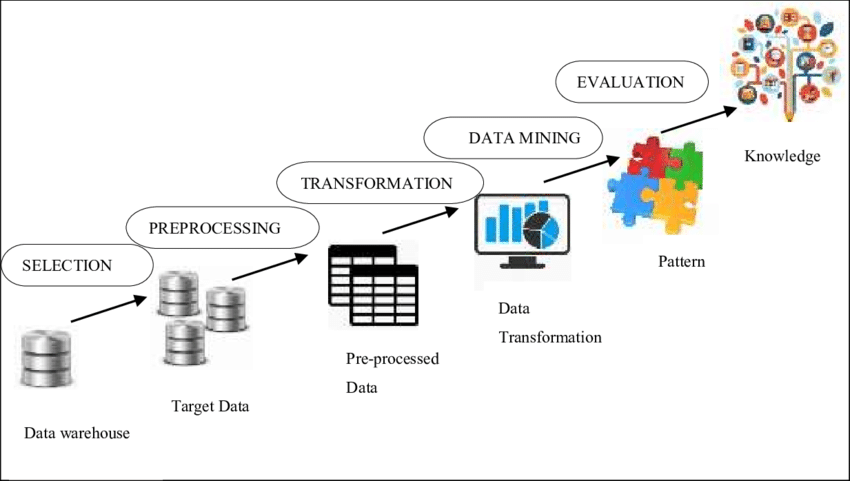
\includegraphics[width=12cm]{kdd-process}}%
\end{figure}

In una prima fase si sviluppa una \textbf{comprensione del dominio} dell'applicazione, delle relative conoscenze di base e degli obiettivi dell'utente finale. Si prosegue creando \textbf{un data set target}, quindi si seleziona un dataset o ci si focalizza su un sotto insieme di variabili o di esempi di dati sui quali deve essere eseguita la scoperta. Una volta selezionati questi dati si passa alla fase di \textbf{pulizia dei dati e preprocessing} nella quale si effettuano svariate operazioni volte a rimuovere il rumore o dei valori anomali, collezionando le informazioni necessarie per modellare o tenere conto del rumore, decidere strategie per gestire i campi di dati mancanti o tenere conto delle informazioni sulla sequenza temporale e delle modifiche note. Successivamente si entra in una fase di \textbf{riduzione e proiezione dei dati}, nella quale si trovano funzioni utili per rappresentare i dati a seconda dell'obiettivo dell'attività. Vengono utilizzati metodi di riduzione o trasformazione multidimensionale per ridurre l'effettivo numero di variabili da considerare o per trovare rappresentazioni di dati invarianti. Conclusa questa attività, si passa alla \textbf{selezione del compito del data mining}, decidendo qual è l'obiettivo del processo KDD, scegliendo tra classificazione, regressione, clustering. 

Definito l'obiettivo si passa alla \textbf{scelta degli algoritmi} di data mining. Vengono selezionati i metodi che verranno utilizzati per ricercare i pattern frequenti all'interno dei dati. Vengono definiti i modelli e i parametri piùù appropriati e si cerca di far corrispondere particolari metodi di data mining con i criteri globali dei processi di KDD. Quindi si entra nella fase di \textbf{Data Mining}, nella quale si ricercano modelli di interesse in una particolare forma rappresentativa.  L'utente può contribuire significativamente in questa fase eseguendo correttamente i passaggi precedenti. Alla fine del processo di data mining, vi è la fase di \textbf{interpretazione dei pattern minati}, nella quale si effettuano le valutazioni sui risultati ottenuti ed eventualmente si ritorna ad iterare su uno degli step precedenti. Infine si \textbf{consolida la conoscenza scoperta}, la conoscenza ottenuta viene incorporata nel sistema per migliorarne le prestazioni o semplicemente si documenta per essere segnalata ad altre parti di interesse. Questa fase include anche il controllo e la risoluzione di particolar conflitti con conoscenze precedentemente estratte o scoperte.

La maggior parte del lavoro nel KDD è focalizzata sullo step del data mining. Anche se gli altri step sono considerati importanti per il successo dell'applicazione del KDD nella pratica. La necessità per una standardizzazione del processo della scoperta della conoscenza ha portato alla definizione dello standard industriale CRISP-DM. L'obiettivo di questo standard è quello di sviluppare un processo neutrale per condurre il KD,  e di definire i compiti, i loro outputs, la terminologia e i problemi tipici di caraterizzazione. 

Il modello di processo CRISP-DM è per la scoperta i conoscenza consiste in sei fasi.

\begin{figure}[h]
\noindent
\makebox[\textwidth]{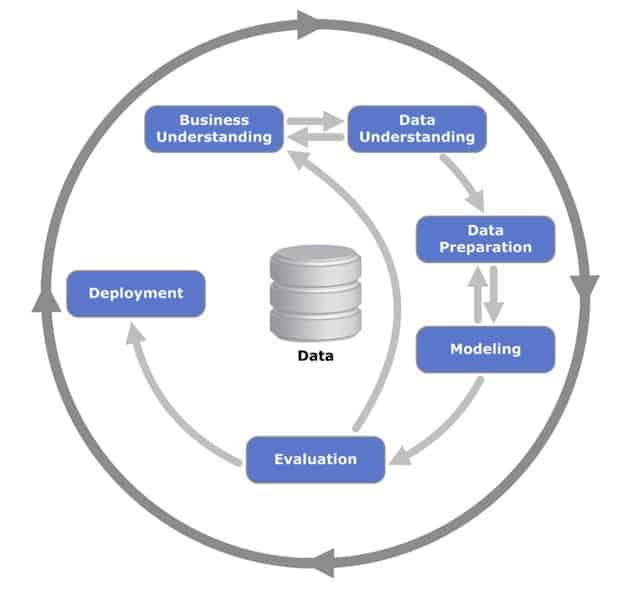
\includegraphics[width=10cm]{crisp-dm-model}}%
\end{figure}

La sequenza delle fasi non è rigida. È possibile spostarsi avanti e indietro tra le diverse fasi a seconda dell'esito di ciascuna fase. Le frecce indicano le dipendenze più importanti/frequenti. Il cerchio esterno simboleggia la natura ciclica di un processo KDD che può continuare dopo l'implementazione di una soluzione. Ogni fase contiene un numero di task che prouce specifici output

\end{document}
